\label{kap-metody}

\subsection {Akustická oscilometrie}
Invazivní metody měření respiračního systému se v současné době nevyužívají. Častěji se využívají metody neinvazivní jako např. spirometrie nebo akustická oscilometrie. Spirometrie je jedna z nejčastěji využívaných metod pro analýzu dýchacího systému, avšak k jejímu provedení je třeba spolupráce pacienta, který musí provádět hluboké nádechy a výdechy.
Akustická oscilometrie (dále AOS) má oproti spirometrii výhodu v tom, že vyžaduje pouze minimální spolupráci pacienta ve smyslu klidného spontánního dýchání. 
Je založená na základě měření impedance dýchacích cest. Výsledkem měření je kombinace hodnot rezistance a reaktance. Souhrnně se tyto dvě hodnoty nazývají impedancí. 

AOS je měřena pomocí přístroje tremoflo C-100. Podstatou funkce tohoto přístroje je akustické vlnění, které je vytvářeno pohybem síta. Akustické vlny jsou odporem dýchacích ces posunuty a deformovány a takto vzniklá oscilační akustická vlna je snímána senzory a počítačově zpracována
 Všechny zaznamenané hodnoty zpracuje software tremoFlo, jenž nakonec vypočítá veličinu impedance respiračního systému $Z_{rs}$. 

\begin{equation}
 \label{rce:1}
  \frac{P(f)}{Q(f)} = Z_{rs}(f) = R_{rs}(f) + j X_{rs}(f) 
\end{equation}
Kde P je tlak, Q je průtok a f je oscilační frekvence. 
Reálná část je označována jako rezistance $R_{rs}$, imaginární část je reaktance $X_{rs}$ a $j = \sqrt{-1}$. 
$R_{rs}$ představuje odpor vůči proudění vzduchu v plicích neboli, kolik tlaku je nutné pro průtok vzduchu dýchacími cestami. $X_{rs}$ znázorňuje při nízkých frekvencích tuhost tkání dýchacích cest.  \cite{Vlcek2018}


Technika nucených oscilací vysílá oscilace o velikosti přibližně \SI{2}{cm} sloupce $H_{2}O$, které se vytvoří v přístroji pomocí reproduktoru a následně se šíří do respiračního systému člověka. Reproduktor vytváří oscilační tlakové vlny na různých frekvencích. Nízké frekvence se šíří hluboko do plic, odkud se následně odrážejí zpátky do přístroje a vyšší frekvence se nedostanou hlouběji do plic, protože se  odrážejí zpátky do přístroje hned z periferních cest dýchacích. Tato skutečnost je daná fyzikálními vlastnostmi lidského těla, především velikostí a tvarem tkáňového složení lidského hrudníku. \cite{Vlcek2018} Frekvencí se k~měření používá devět (\SI{5}{Hz}, \SI{11}{Hz}, \SI{13}{Hz}, \SI{17}{Hz}, \SI{19}{Hz}, \SI{23}{Hz}, \SI{31}{Hz} a  \SI{37}{Hz}). 

V přístroji je umístěn snímač tlaku a průtoku a ty přeměřují inspirační a expirační tlak plic a průtok dýchacích cest. 

Respirační impedance je součet rezistance a reaktance a je vypočítán z poměru tlaku  $P$ ku průtoku $Q$ u každé oscilační frekvence $f$. \cite{Vlcek2018}

\begin{equation}
	\label{rce:2}
	Z_{rs}(f) = \frac{P(f)}{Q(f)}
\end{equation}


V tomto projektu byl použit přístroj tremoflo C-100, který měří impedanci na frekvencích \SI{5}{Hz}-\SI{37}{Hz}. Reaktance a rezistance jsou označovány $X$ a $R$ a v dolním indexu se nachází velikost frekvence na které byly měřeny, tj. např. pro frekvenci \SI{5}{Hz} bude vypadat označení reaktance $X_5$ a rezistence $R_5$. 


Rezistance ($R_{rs}$) je veličina, která určuje centrální a periferní velikost odporu dýchacích cest. Velikost odporu dýchacích cest je zapříčiněna průchodností tlakové vlny vygenerované zařízením. Základní pevná frekvence pro oscilující tlaky je 5~Hz. Další frekvence se odvozují od tohoto základu odvozují. Do odvozených skupin frekvencí patří nízkofrekvenční signály (\SI{5}{Hz}-\SI{17}{Hz}), které se dostávají do obvodu centra plic, a vysokofrekvenční signály (\SI{19}{Hz}-\SI{37}{Hz}), jež pronikají pouze do proximálních dýchacích cest. 

Reaktance je imaginární část impedance. Jedná se o měřítko tuhosti plic, obzvlášť při nižších frekvencích. Toto měření vyplývá z pohybu vzduchu  a zpětné elasticitě plicní tkáně. Vzhledem k elastickým vlastnostem se tedy plíce při nízkých frekvencích pasivně rozšiřují a dochází tak k malému zpětnému rázu. Se zvyšující se energii dochází k přechodu plic z pasivního roztažení na aktivní. Čím vyšší je frekvence, tím víc energie putuje do plicního systému. 

Poddajnost je fyzikální veličina, která popisuje míru schopnosti tělesa měnit tvar působením vnější síly při pružné deformaci. \cite{Poddajnost}

Inertance je fyzikální veličina, která funguje jako měřítko odporu proti změně rychlosti toku plynu do plic. \cite{Inertance}

\subsection{Kalibrace zařízení tremoflo}\label{kalibrace}
Přístroj, kterým bylo měření prováděno se nazývá TremoFlo C-100 (Thorasys Thoracic Medical Systems Inc., Kanada). Zařízení vyžaduje kalibraci před každým použitím. Kalibrace se provádí pomocí kalibrační zátěže, která je součástí balení. Kalibrační zátěž je označena konkrétním kódem, který se vloží do systému, následně  se nasadí na přenosný díl a spustí se kalibrace. Pro spolehlivé a přesné měření musí být přesnost 
v rozmezí \SI{10}{\%} nebo $\SI{0,1}{cm \cdot H_{2}O \cdot s/L}$. Pokud je tato podmínka splněna může se provést měření. \cite{Vlcek2018}

\subsection{Sestavení modelu}
Respirační systém se skládá se z pravé a levé plíce a průdušnic. Model respiračního systému  byl sestrojen pomocí mechanických analogií, skleněné nádoby, plastové trubice a průtočného rezistoru. Byly použity dvě velikosti nádob \SI{35}{L} a \SI{54}{L}, tři délky plastové trubice, \SI{20}{cm},  \SI{40}{cm},  \SI{60}{cm}  a tři různé parabolické rezistory PneuFlo Rp~5, Rp~20 a Rp~50 (Michigan Instruments, Michigan). 
Tremoflo C-100 je přístroj, který superponuje oscilace na spontánní dýchání člověka, tudíž model plic musí simulovat dýchání. Toto bylo vyřešeno mechanicky stříkačkou, která byla nastavena na  \SI{1}{L}, tudíž při každém stlačení vpustila do systému  \SI{1}{L} vzduchu. 
Postupně pomocí těchto součástek byly sestrojeny všechny kombinace respiračního systému a změřena odezva přístroje tremoflo C-100.

\begin{figure}[!h]
			\centering
 			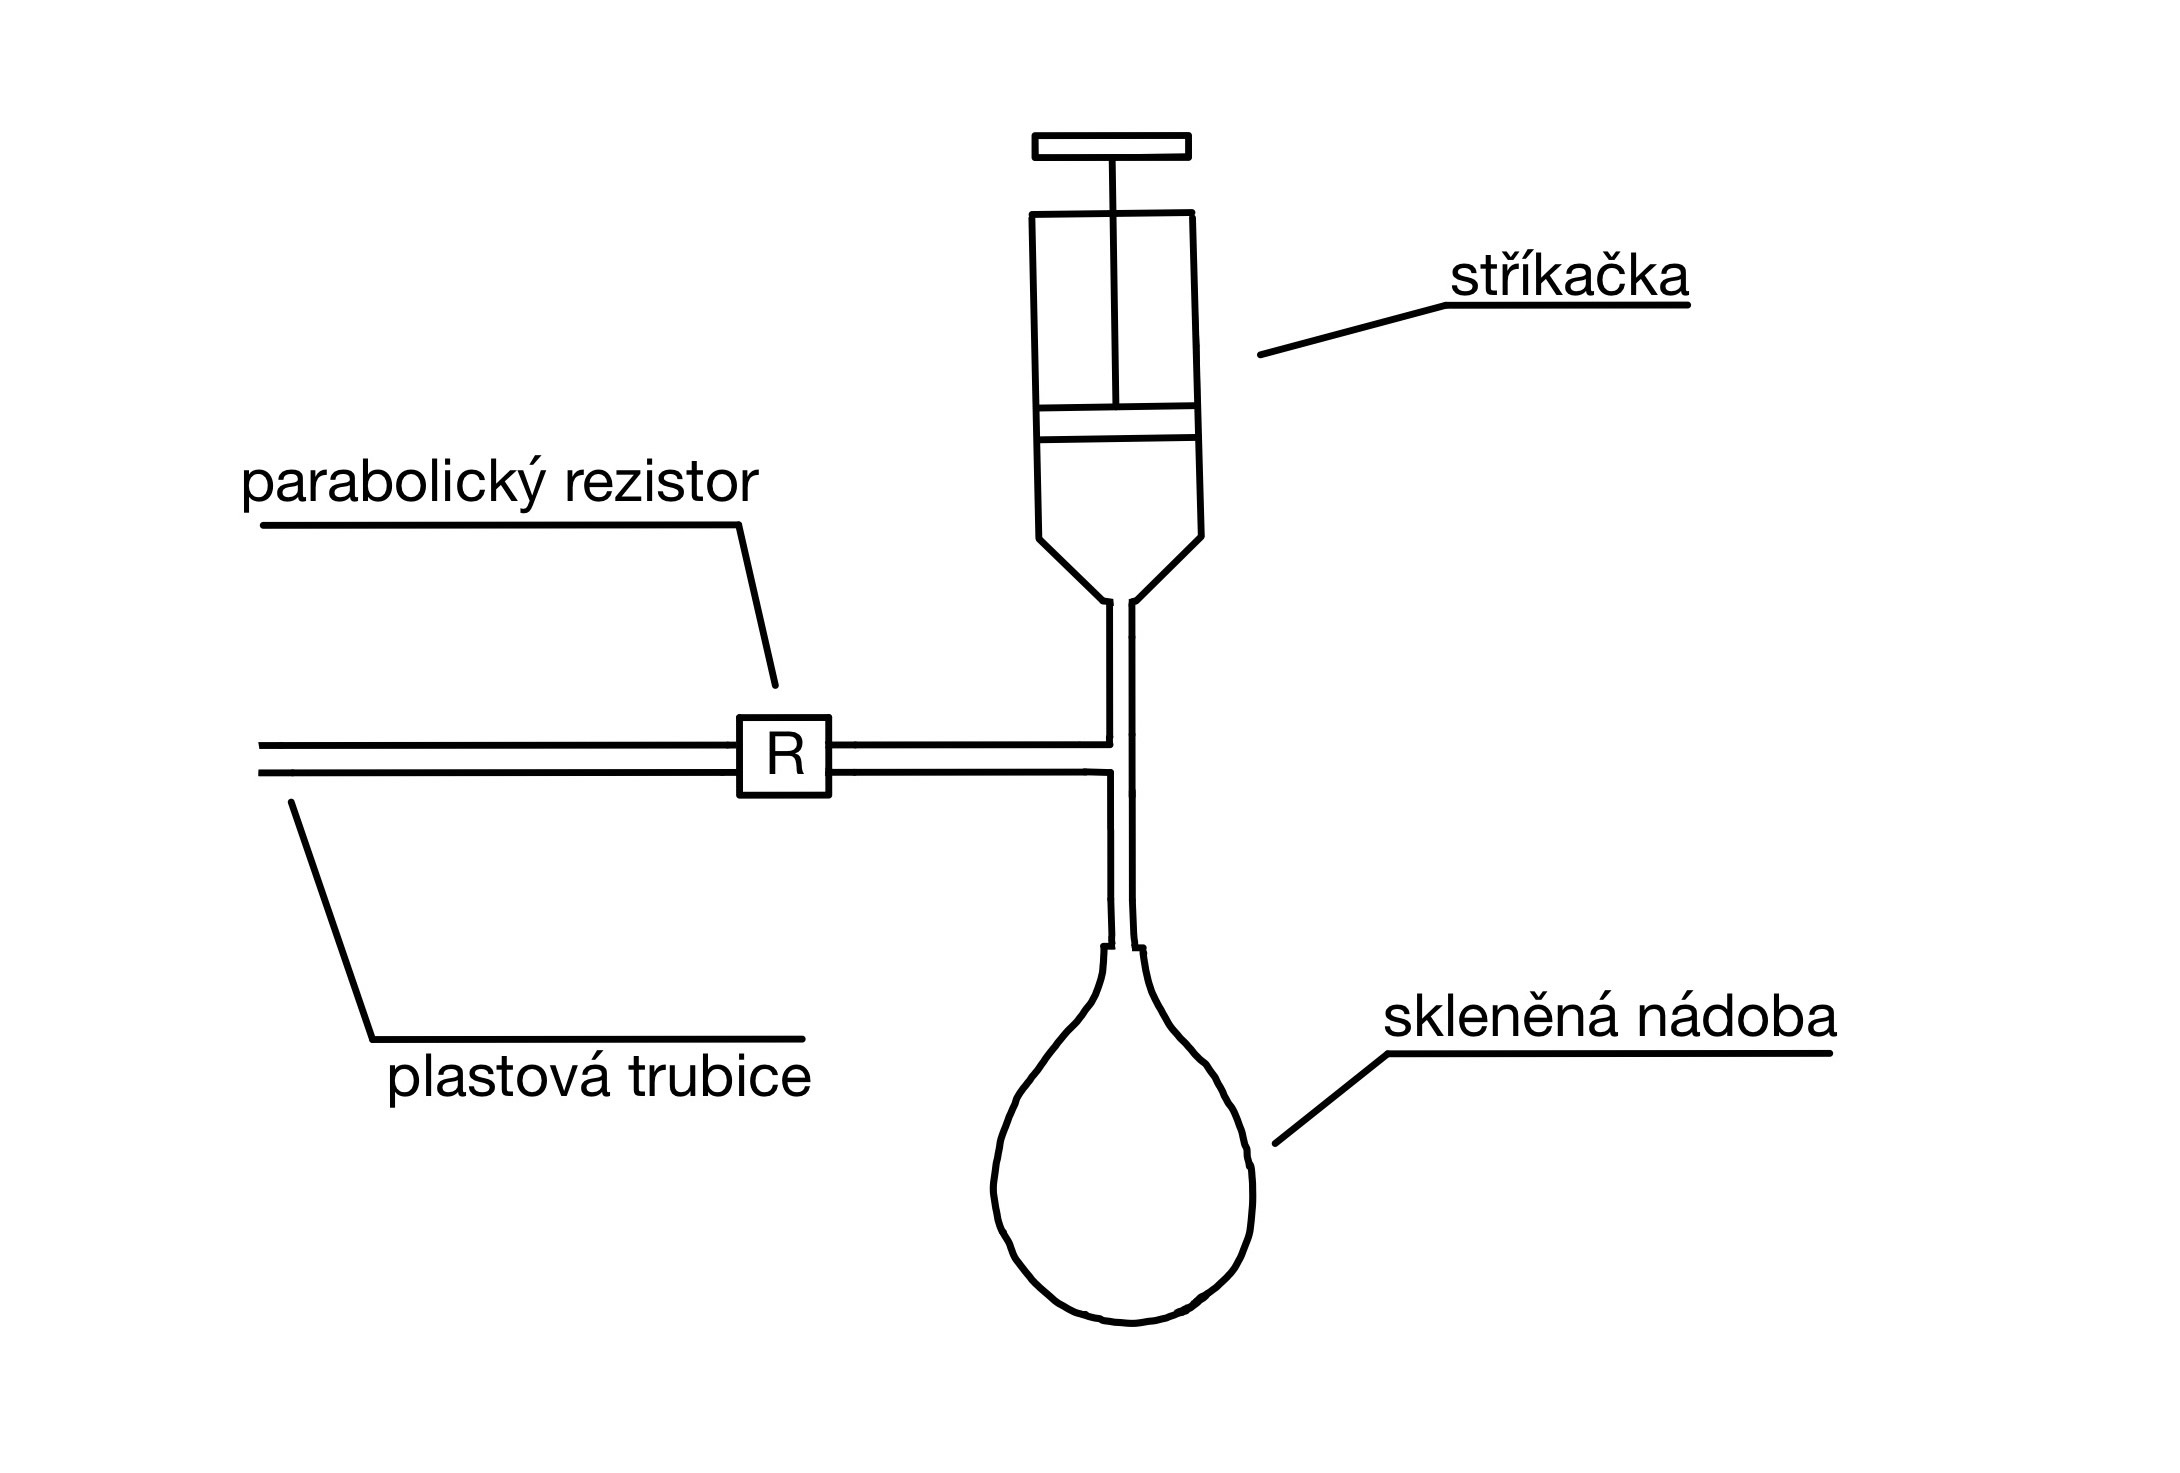
\includegraphics[width=1\textwidth]{schema}
			\caption{Schéma modelu respiračního systému}
			 \label{obrazekschema}
 \end{figure}

\subsection{Průběh měření}
Měření bylo prováděno v laboratoři pomocí přístroje tremoflo C-100 od firmy Thorasys. K měření byl třeba počítač s nainstalovaným softwarem pro tento přístroj. Na software tremoflo je třeba mít licenci, tudíž měření bylo možné provádět pouze na konkrétním počítači, kde je licence nainstalována.  Nejprve se přístroj i počítač zapojil do elektrické sítě a zapnul. Přístroj tremoflo C-100 se propojí s počítačem pomocí USB kabelu a po startu ovládacího software je potřeba provést kalibraci pomocí kalibrační zátěže, popis kalibrace je v podkapitole \ref{kalibrace}). Software nemá testovací režim, tudíž před měřením je třeba vytvořit kartu fiktivního pacienta. Do ní je třeba vyplnit  jméno, příjmení a věk pacienta. Po sestavení první kombinace modelu a vytvoření fiktivního pacienta se může přejít k měření. Každé měření probíhalo  \SI{16}{s} během kterých byla mechanicky stlačována střička, která do systému vháněla vzduch. Po  \SI{16}{s} přístroj data uložil a měření se opakovalo 3x kvůli snížení chyb a následnému průměrování. Po 3~měřeních jedné kombinace se jeden článek modelu, průtočný odpor, délka plastové trubice nebo velikost skleněné nádoby vyměnila a měření se opakovalo. Tímhle způsobem se vystřídaly všechny kombinace. Všechny data byla uložena v systému a potom se z~nich vygenerovala tabulka

